% Options for packages loaded elsewhere
\PassOptionsToPackage{unicode}{hyperref}
\PassOptionsToPackage{hyphens}{url}
%
\documentclass[
  11pt,
]{article}
\usepackage{amsmath,amssymb}
\usepackage{lmodern}
\usepackage{iftex}
\ifPDFTeX
  \usepackage[T1]{fontenc}
  \usepackage[utf8]{inputenc}
  \usepackage{textcomp} % provide euro and other symbols
\else % if luatex or xetex
  \usepackage{unicode-math}
  \defaultfontfeatures{Scale=MatchLowercase}
  \defaultfontfeatures[\rmfamily]{Ligatures=TeX,Scale=1}
\fi
% Use upquote if available, for straight quotes in verbatim environments
\IfFileExists{upquote.sty}{\usepackage{upquote}}{}
\IfFileExists{microtype.sty}{% use microtype if available
  \usepackage[]{microtype}
  \UseMicrotypeSet[protrusion]{basicmath} % disable protrusion for tt fonts
}{}
\makeatletter
\@ifundefined{KOMAClassName}{% if non-KOMA class
  \IfFileExists{parskip.sty}{%
    \usepackage{parskip}
  }{% else
    \setlength{\parindent}{0pt}
    \setlength{\parskip}{6pt plus 2pt minus 1pt}}
}{% if KOMA class
  \KOMAoptions{parskip=half}}
\makeatother
\usepackage{xcolor}
\IfFileExists{xurl.sty}{\usepackage{xurl}}{} % add URL line breaks if available
\IfFileExists{bookmark.sty}{\usepackage{bookmark}}{\usepackage{hyperref}}
\hypersetup{
  pdftitle={Lab 2: Exploration by visualization: the streaming movies dataset},
  pdfauthor={Minsu Kang and Minsung Kim},
  hidelinks,
  pdfcreator={LaTeX via pandoc}}
\urlstyle{same} % disable monospaced font for URLs
\usepackage[margin=1in]{geometry}
\usepackage{color}
\usepackage{fancyvrb}
\newcommand{\VerbBar}{|}
\newcommand{\VERB}{\Verb[commandchars=\\\{\}]}
\DefineVerbatimEnvironment{Highlighting}{Verbatim}{commandchars=\\\{\}}
% Add ',fontsize=\small' for more characters per line
\usepackage{framed}
\definecolor{shadecolor}{RGB}{248,248,248}
\newenvironment{Shaded}{\begin{snugshade}}{\end{snugshade}}
\newcommand{\AlertTok}[1]{\textcolor[rgb]{0.94,0.16,0.16}{#1}}
\newcommand{\AnnotationTok}[1]{\textcolor[rgb]{0.56,0.35,0.01}{\textbf{\textit{#1}}}}
\newcommand{\AttributeTok}[1]{\textcolor[rgb]{0.77,0.63,0.00}{#1}}
\newcommand{\BaseNTok}[1]{\textcolor[rgb]{0.00,0.00,0.81}{#1}}
\newcommand{\BuiltInTok}[1]{#1}
\newcommand{\CharTok}[1]{\textcolor[rgb]{0.31,0.60,0.02}{#1}}
\newcommand{\CommentTok}[1]{\textcolor[rgb]{0.56,0.35,0.01}{\textit{#1}}}
\newcommand{\CommentVarTok}[1]{\textcolor[rgb]{0.56,0.35,0.01}{\textbf{\textit{#1}}}}
\newcommand{\ConstantTok}[1]{\textcolor[rgb]{0.00,0.00,0.00}{#1}}
\newcommand{\ControlFlowTok}[1]{\textcolor[rgb]{0.13,0.29,0.53}{\textbf{#1}}}
\newcommand{\DataTypeTok}[1]{\textcolor[rgb]{0.13,0.29,0.53}{#1}}
\newcommand{\DecValTok}[1]{\textcolor[rgb]{0.00,0.00,0.81}{#1}}
\newcommand{\DocumentationTok}[1]{\textcolor[rgb]{0.56,0.35,0.01}{\textbf{\textit{#1}}}}
\newcommand{\ErrorTok}[1]{\textcolor[rgb]{0.64,0.00,0.00}{\textbf{#1}}}
\newcommand{\ExtensionTok}[1]{#1}
\newcommand{\FloatTok}[1]{\textcolor[rgb]{0.00,0.00,0.81}{#1}}
\newcommand{\FunctionTok}[1]{\textcolor[rgb]{0.00,0.00,0.00}{#1}}
\newcommand{\ImportTok}[1]{#1}
\newcommand{\InformationTok}[1]{\textcolor[rgb]{0.56,0.35,0.01}{\textbf{\textit{#1}}}}
\newcommand{\KeywordTok}[1]{\textcolor[rgb]{0.13,0.29,0.53}{\textbf{#1}}}
\newcommand{\NormalTok}[1]{#1}
\newcommand{\OperatorTok}[1]{\textcolor[rgb]{0.81,0.36,0.00}{\textbf{#1}}}
\newcommand{\OtherTok}[1]{\textcolor[rgb]{0.56,0.35,0.01}{#1}}
\newcommand{\PreprocessorTok}[1]{\textcolor[rgb]{0.56,0.35,0.01}{\textit{#1}}}
\newcommand{\RegionMarkerTok}[1]{#1}
\newcommand{\SpecialCharTok}[1]{\textcolor[rgb]{0.00,0.00,0.00}{#1}}
\newcommand{\SpecialStringTok}[1]{\textcolor[rgb]{0.31,0.60,0.02}{#1}}
\newcommand{\StringTok}[1]{\textcolor[rgb]{0.31,0.60,0.02}{#1}}
\newcommand{\VariableTok}[1]{\textcolor[rgb]{0.00,0.00,0.00}{#1}}
\newcommand{\VerbatimStringTok}[1]{\textcolor[rgb]{0.31,0.60,0.02}{#1}}
\newcommand{\WarningTok}[1]{\textcolor[rgb]{0.56,0.35,0.01}{\textbf{\textit{#1}}}}
\usepackage{graphicx}
\makeatletter
\def\maxwidth{\ifdim\Gin@nat@width>\linewidth\linewidth\else\Gin@nat@width\fi}
\def\maxheight{\ifdim\Gin@nat@height>\textheight\textheight\else\Gin@nat@height\fi}
\makeatother
% Scale images if necessary, so that they will not overflow the page
% margins by default, and it is still possible to overwrite the defaults
% using explicit options in \includegraphics[width, height, ...]{}
\setkeys{Gin}{width=\maxwidth,height=\maxheight,keepaspectratio}
% Set default figure placement to htbp
\makeatletter
\def\fps@figure{htbp}
\makeatother
\setlength{\emergencystretch}{3em} % prevent overfull lines
\providecommand{\tightlist}{%
  \setlength{\itemsep}{0pt}\setlength{\parskip}{0pt}}
\setcounter{secnumdepth}{-\maxdimen} % remove section numbering
\ifLuaTeX
  \usepackage{selnolig}  % disable illegal ligatures
\fi

\title{Lab 2: Exploration by visualization: the streaming movies
dataset}
\author{Minsu Kang and Minsung Kim}
\date{2022-06-30}

\begin{document}
\maketitle

\begin{center}\rule{0.5\linewidth}{0.5pt}\end{center}

\hypertarget{visualization-by-example}{%
\subsection{Visualization by example}\label{visualization-by-example}}

\hypertarget{exercise-1}{%
\subsubsection{Exercise 1}\label{exercise-1}}

\begin{Shaded}
\begin{Highlighting}[]
\FunctionTok{View}\NormalTok{(streaming)}
\FunctionTok{qplot}\NormalTok{(}\AttributeTok{x=}\NormalTok{im\_db, }\AttributeTok{binwidth=}\FloatTok{0.5}\NormalTok{, }\AttributeTok{data=}\NormalTok{streaming)}
\end{Highlighting}
\end{Shaded}

\begin{center}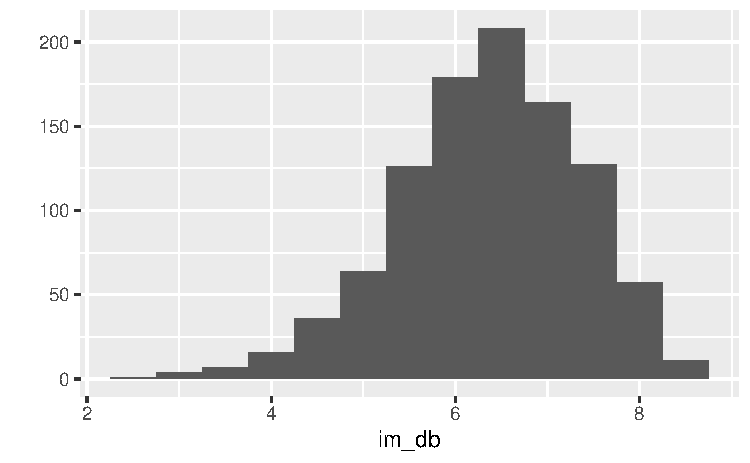
\includegraphics[width=0.8\linewidth]{lab02_files/figure-latex/unnamed-chunk-1-1} \end{center}

\begin{itemize}
\tightlist
\item
  Question1 The View function shows whole data on Console window. The
  histogram with qplot function showed in plots window. The histogram
  shows the shape of distribution and density of im\_db.
\end{itemize}

\hypertarget{exercise-2}{%
\subsubsection{Exercise 2}\label{exercise-2}}

\begin{Shaded}
\begin{Highlighting}[]
\FunctionTok{qplot}\NormalTok{(}\AttributeTok{x=}\NormalTok{im\_db, }\AttributeTok{binwidth=}\FloatTok{0.5}\NormalTok{, }\AttributeTok{fill=}\NormalTok{main\_language, }\AttributeTok{data=}\NormalTok{streaming)}
\end{Highlighting}
\end{Shaded}

\begin{center}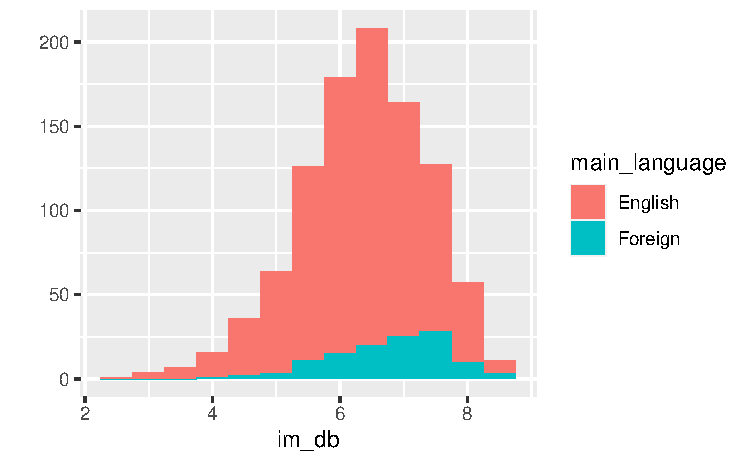
\includegraphics[width=0.8\linewidth]{lab02_files/figure-latex/unnamed-chunk-2-1} \end{center}

\begin{itemize}
\item
  Question1 It fill out the bar graph with color.
\item
  Question2 Most of movies made by english.
\end{itemize}

\hypertarget{exercise-3}{%
\subsubsection{Exercise 3}\label{exercise-3}}

\begin{itemize}
\item
  Question1 English and Foreign IMDB shows left-skewed distribution, and
  centered around 6 to 8. The average between English and Foregin film
  have a substantial difference.
\item
  Question2 Yes. It is hard to foray into American movie market as a
  Foreign film. So, only who has perfect stories, or great creativity
  foreign films can success and can be created by IMDB. So only the
  famous one can translated and rated. Plus, for the translating, it
  costs more than English movie. However, English movies have low
  obstacles to entry and rated, and even it is small films it is easy to
  rated. So the quality of movie is not guaranteed.
\end{itemize}

\hypertarget{exercise-4}{%
\subsubsection{Exercise 4}\label{exercise-4}}

\begin{Shaded}
\begin{Highlighting}[]
\FunctionTok{qplot}\NormalTok{(}
  \AttributeTok{x =}\NormalTok{ im\_db, }
  \AttributeTok{binwidth =} \FloatTok{0.5}\NormalTok{, }
  \AttributeTok{facets =} \SpecialCharTok{\textasciitilde{}}\NormalTok{ age,}
  \AttributeTok{data =}\NormalTok{ streaming)}
\end{Highlighting}
\end{Shaded}

\begin{center}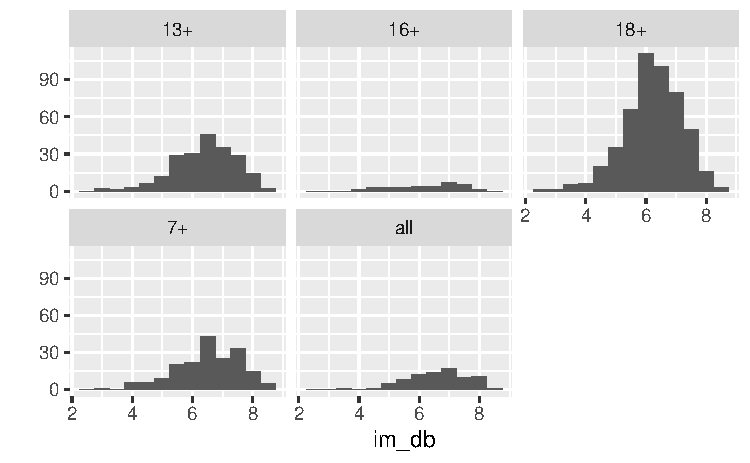
\includegraphics[width=0.8\linewidth]{lab02_files/figure-latex/unnamed-chunk-3-1} \end{center}

\begin{itemize}
\item
  Question1 There are 5 facets.
\item
  Question2 The facets represent IMDB rating depends on age(film
  rating).
\item
  Question3 R rated movie distribution facet contains most movies.
\end{itemize}

\hypertarget{exercise-5}{%
\subsubsection{Exercise 5}\label{exercise-5}}

\begin{Shaded}
\begin{Highlighting}[]
\FunctionTok{qplot}\NormalTok{(}\AttributeTok{x=}\NormalTok{rotten\_tomatoes, }\AttributeTok{y=}\NormalTok{im\_db, }\AttributeTok{data=}\NormalTok{streaming)}
\end{Highlighting}
\end{Shaded}

\begin{center}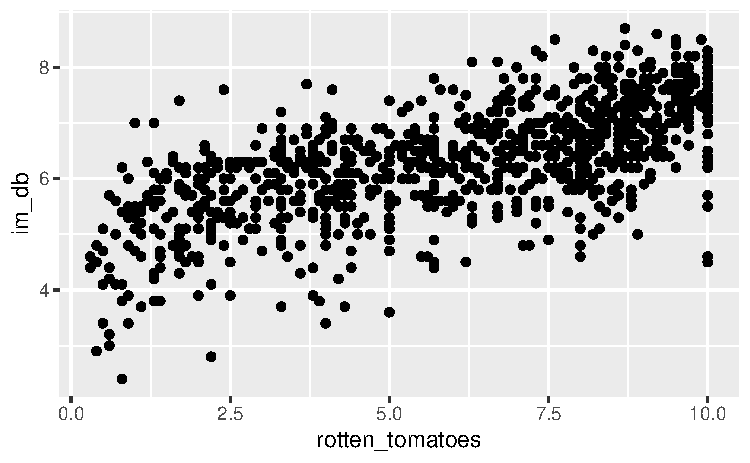
\includegraphics[width=0.8\linewidth]{lab02_files/figure-latex/unnamed-chunk-4-1} \end{center}

\begin{itemize}
\tightlist
\item
  Question 1 When Rotten\_tomatoes going up, The IMDB also rated
  high(positive, linear relationship).
\end{itemize}

\hypertarget{exercise-6}{%
\subsubsection{Exercise 6}\label{exercise-6}}

\begin{Shaded}
\begin{Highlighting}[]
\FunctionTok{qplot}\NormalTok{(}\AttributeTok{x=}\NormalTok{rotten\_tomatoes, }\AttributeTok{y=}\NormalTok{im\_db, }\AttributeTok{data=}\NormalTok{streaming, }\AttributeTok{color=}\NormalTok{main\_language)}
\end{Highlighting}
\end{Shaded}

\begin{center}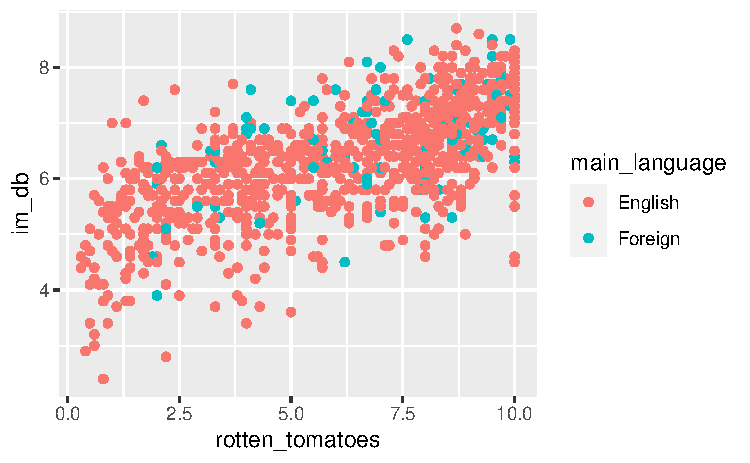
\includegraphics[width=0.8\linewidth]{lab02_files/figure-latex/unnamed-chunk-5-1} \end{center}

\begin{itemize}
\tightlist
\item
  Question 1 English movie scattered all over the rates, but Foreign
  films dense in right, upper quadrant.
\end{itemize}

\hypertarget{exercise-7}{%
\subsubsection{Exercise 7}\label{exercise-7}}

\begin{Shaded}
\begin{Highlighting}[]
\FunctionTok{qplot}\NormalTok{(}\AttributeTok{x=}\NormalTok{rotten\_tomatoes, }\AttributeTok{y=}\NormalTok{im\_db, }\AttributeTok{data=}\NormalTok{streaming, }\AttributeTok{facets=} \SpecialCharTok{\textasciitilde{}}\NormalTok{age)}
\end{Highlighting}
\end{Shaded}

\begin{center}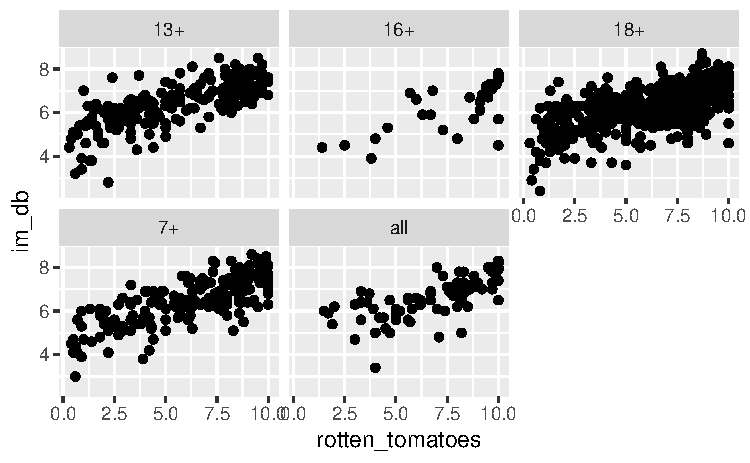
\includegraphics[width=0.8\linewidth]{lab02_files/figure-latex/unnamed-chunk-6-1} \end{center}

\begin{itemize}
\tightlist
\item
  Question 1 It shows same data, but divided by ages(film ratings).
\end{itemize}

\hypertarget{exercise-8}{%
\subsubsection{Exercise 8}\label{exercise-8}}

\begin{Shaded}
\begin{Highlighting}[]
\FunctionTok{qplot}\NormalTok{(}
  \AttributeTok{x =}\NormalTok{ rotten\_tomatoes, }
  \AttributeTok{y =}\NormalTok{ im\_db, }
  \AttributeTok{geom =} \StringTok{"smooth"}\NormalTok{, }
  \AttributeTok{method =} \StringTok{"lm"}\NormalTok{, }
  \AttributeTok{data =}\NormalTok{ streaming}
\NormalTok{  )}
\end{Highlighting}
\end{Shaded}

\begin{verbatim}
## `geom_smooth()` using formula 'y ~ x'
\end{verbatim}

\begin{center}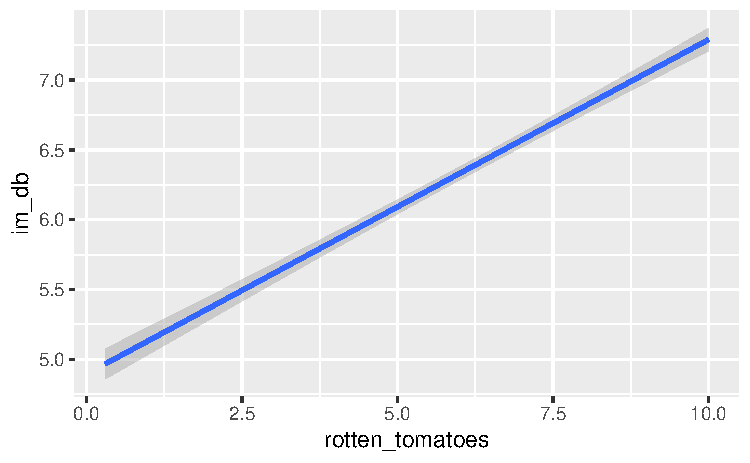
\includegraphics[width=0.8\linewidth]{lab02_files/figure-latex/unnamed-chunk-7-1} \end{center}

\begin{itemize}
\tightlist
\item
  Question 1 It follows same linear trends.
\end{itemize}

\hypertarget{exercise-9}{%
\subsubsection{Exercise 9}\label{exercise-9}}

\begin{Shaded}
\begin{Highlighting}[]
\FunctionTok{qplot}\NormalTok{(}
  \AttributeTok{x =}\NormalTok{ rotten\_tomatoes, }
  \AttributeTok{y =}\NormalTok{ im\_db, }
  \AttributeTok{geom =} \FunctionTok{c}\NormalTok{(}\StringTok{"smooth"}\NormalTok{,}\StringTok{"point"}\NormalTok{), }
  \AttributeTok{method =} \StringTok{"lm"}\NormalTok{, }
  \AttributeTok{data =}\NormalTok{ streaming}
\NormalTok{  )}
\end{Highlighting}
\end{Shaded}

\begin{verbatim}
## Warning: Ignoring unknown parameters: method
\end{verbatim}

\begin{verbatim}
## `geom_smooth()` using formula 'y ~ x'
\end{verbatim}

\begin{center}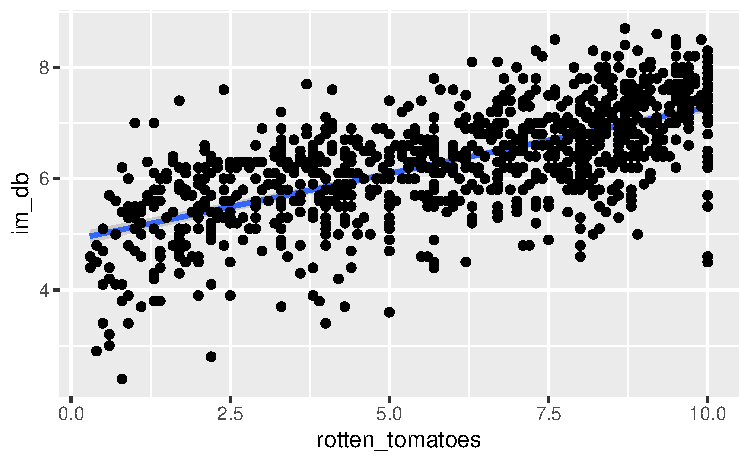
\includegraphics[width=0.8\linewidth]{lab02_files/figure-latex/unnamed-chunk-8-1} \end{center}

\end{document}
